\chapter{Mätteknik}

\emph{I forskning, utveckling och produktion är mätning en hörnpelare
  i verksamheten. Även inom mättekniken sker en snabb utveckling och
  digitaltekniken kommer alltmer till användning, men grunderna för
  mätning är desamma. I detta kapitel behandlas de viktigaste
  mättekniska begreppen som radioamatörer kan behöva känna till.}

\section{Att mäta}
\textbf{HAREC
  a.\ref{HAREC.a.8.1}\label{myHAREC.a.8.1}
  a.\ref{HAREC.a.8.1.1.1}\label{myHAREC.a.8.1.1.1}
}

\subsection{Mäta likspänning}
\index{inre resistans}

Vid spänningsmätning bestämmer man potentialskillnaden -- spänningen --
mellan två punkter.
Om det finns en spänning, så flyter en motsvarande (mät)ström genom
instrumentet som presenterar mätströmmen som en spänning.

Mätströmmen påverkar emellertid spänningsfördelningen i kretsen och då
uppstår ett mätfel, vilket inte framgår av det visade mätvärdet.
Med kännedom om kretsens och instrumentets data kan man dock beräkna mätfelet.
En voltmeter ska ha hög \emph{inre resistans} för att mätfelet ska bli litet.

Endast vid mycket noggrann mätning kan man behöva räkna om det visade
mätvärdet med hänsyn till voltmeterns inre resistans och
förkopplingsresistansen -- om en sådan används).

\textbf{På grund av den höga inre resistansen är en voltmeter endast lämpad
  för spänningsmätning -- INTE för direkt strömmätning!}

\subsubsection{Utöka mätområdet för en voltmeter}

Med hjälp av förkopplingsresistor i serie med voltmetern kan man mäta
högre spänning än den som voltmetern är gjord för.
Spänningen fördelas då proportionellt mellan förkopplingsresistorns resistans
och instrumentets inre resistans.
Ett exempel på detta finns i bild \ref{fig:BildII3-01}.

När förkopplingsresistor används måste mätvärdet räknas om med en
skalfaktor eller en skala med motsvarande gradering användas.
En voltmeter med valbar förkopplingsresistor kan därför har flera skalor.
I digitala voltmetrar anpassas ''skalan'' oftast automatiskt.

\subsubsection{Inre resistansens inverkan}
\textbf{
HAREC a.\ref{HAREC.a.8.1.2.3}\label{myHAREC.a.8.1.2.3}
}
\index{inre resistans}

Vid mätning av spänning kommer den inre resistansen hos voltmetern att lasta
kretsen, och därmed sänka spänningen och därmed kommer den uppmätta spänningen
vara lägre än den faktiska spänningen utan mätinstrumentet.

I gamla tider var den inre resistansen relativt låg, varvid påverkan blev
större än med moderna instrument.
Dock kan även moderna instrument påverka mätresultatet i kretsar som har väldigt
hög impedans.

\subsection{Mäta likström}
\index{strömmätning}
\index{inre resistans}

Vid \emph{strömmätning} bestämmer man strömstyrkan i en gren av en elektriskt
strömkrets.
Amperemetern ska kopplas i serie med den aktuella strömgrenen.
Det visade mätvärdet motsvarar strömstyrkan.
Amperemeterns inre resistans adderas emellertid till resistansen i strömgrenen
och då uppstår ett mätfel.
En amperemeter ska ha låg inre resistans för att mätfelet ska bli litet.

Endast vid mycket noggrann mätning kan man behöva räkna om det visade
mätvärdet med hänsyn till amperemeterns inre resistans och resistansen
i strömshunten -- om en sådan används.

\textbf{På grund av den låga inre resistansen ska en amperemeter
  ALDRIG användas för spänningsmätning. Då förstörs den!}

\subsubsection{Utöka mätområdet för en amperemeter}

Med en strömshunt (en resistor parallellt) över amperemetern kan man
mäta högre ström än den som amperemetern är gjord för.

Shunten dimensioneras så att större delen av strömmen leds förbi amperemetern.
Kvar är den mätström som behövs för att amperemetern ska göra fullt utslag.

Mätströmmen fördelar sig omvänt proportionellt mot instrumentets och
shuntens resistanser.

När en strömshunt används måste mätvärdet räknas om med en skalfaktor
eller en skala med motsvarande gradering användas.
En amperemeter med valbar shuntresistor kan därför har flera skalor.
I digitala amperemetrar anpassas ''skalan'' oftast automatiskt.

\subsection{Mäta växelspänning och växelström}

Grunderna för mätning av växelspänning och växelström är samma som för
likspänning och likström, men att bland annat en instrumentlikriktare oftast
behövs.

Beroende på frekvensen i strömkretsen och vilket slags värde man vill
mäta, används olika instrument.

Olika typer av instrument ger olika möjligheter, men också begränsningar.

\emph{Mjukjärnsinstrument} utan likriktare kan mäta växelströmmar ner
till ca 50~mA och upp till ca 10~A.
Frekvensen får dock inte vara högre än ca 100~Hz.

\emph{Vridspoleinstrument} används dels direkt för likströmsmätning
och dels med likriktare även för växelströmsmätning.

Vridspoleinstrument med likriktare används ofta för frekvenser upp
till ca 10~kHz och strömmar ner till 0,1~mA.
Noggrannheten är sällan bättre än 1,5~\% av fullt utslag.

Beroende på funktionsprincipen kan det skilja på hur instrument mäter,
vilket nödvändigtvis inte är detsamma som hur mätvärdet presenteras.

Mjukjärnsinstrument mäter effektivvärdet av en växelström medan ett
vridspoleinstrument med likriktare mäter likriktade medelvärdet.
Som exempel kan skalan i ett instrument med likriktare även graderas för
effektivvärdet för sinusformade förlopp.

För mätning av växelström används vanligen instrument med likriktare,
men för HF även instrument med termokors, vilka bygger på
termogalvanisk spänning mellan metaller.

\subsubsection{Frekvensens inverkan}
\textbf{
HAREC a.\ref{HAREC.a.8.1.2.1}\label{myHAREC.a.8.1.2.1}
}

Frekvensen på den mätta signalen inverkar mer eller mindre på mätresultatet.
Till en del beror det på den instrumenttyp, som används.
En faktor är instrumentets gränsfrekvens, det vill säga hur högt i frekvens som
instrumentet fortfarande är rimligt rättvisande.
Detta kallas instrumentets bandbredd, vilken bör vara dokumenterad.

\subsubsection{Vågformens inverkan}
\textbf{
HAREC a.\ref{HAREC.a.8.1.2.2}\label{myHAREC.a.8.1.2.2}
}

Även formen på den signal som mäts inverkar på mätresultatet och det
är viktigt att veta för vilken vågform som instrumentet presenterar mätvärdet.
Det vanligaste är att vågen förutsätts vara sinusformad, vilket ofta inte är
fallet i praktiken.
Det innebär att fel värde presenteras om vågformen är en annan än den
förutsatta.

\subsection{Mäta resistans}
\textbf{
HAREC a.\ref{HAREC.a.8.1.3}\label{myHAREC.a.8.1.3}
}

Mätning av resistans är enklast att göra på en fristående komponent,
medan man vid mätning på en resistor i en strömkrets också måste ta
hänsyn till att andra komponenter i kretsen kan påverka mätresultatet.

Resistans kan mätas på flera sätt.
Det grundläggande är att mäta strömmen genom resistorn och spänningen över den
och sedan beräkna resistansen med Ohms lag.

Den vanligaste metoden är att använda en modern multimeter som kan mäta
resistans direkt.
En del kräver att man ställer in området för resistans, medan andra
kan göra det automatiskt.

Precisionsmätning av motstånd kan göras av mer avancerade instrument
där man använder 4 punktsmätning.
För 4 punktsmätning så är ström och spänninganslutningarna separerade
så att anslutningsledningarnas resistans inte ger spänning som inkluderas
i den mätta resistansen.
Istället så mäts spänningen så nära som möjligt på själva mätobjektet,
medan spänningsförlusten för strömledarna därmed kan elimineras.
Denna mätmetod är relevant framförallt för lågohmiga motstånd.

\subsection{Mäta effekt}
\textbf{
HAREC a.\ref{HAREC.a.8.1.4}\label{myHAREC.a.8.1.4}
}
\label{mätaeffekt}
\index{PEP}
\index{Peak Envelope Power (PEP)}
\index{effekt!Peak Envelope Power (PEP)}

Effektformler vid lik- och växelström (medel-, effektiv- och toppvärden)

Vid likström:

\(
P = U \cdot I \quad \text{[W (watt)]} \quad \text{dvs. Joules lag} \\
\)

Vid sinusformad växelström och resistiva belastningar:
För PEP-effekt se även avsnitt \ref{PEP-effekt}

\(
\begin{array}{ll}
\text{effektivvärde} \quad P & = \dfrac{U^2}{R} \\
&\\
\text{toppvärde}     \quad P_{PEP} & = \dfrac{U_{max}^2}{R}
\end{array}
\)

U = spänningens effektivvärde
R = resistansen

\subsection{Sändareffekt}

En sändares effekt kan mätas på olika sätt.
Den metod att mäta \emph{uteffekt} som är relevanta för radioamatören är
toppvärdeskännande sådana för mätning av p.e.p.
I föreskrifterna används sändareffekten p.e.p. som uteffekt.
Därvid måste även p.e.p. avses, fastän det inte uttryckligen uttalas.

Observera, att radioamatören måste beakta EMC-lagen.
Se vidare kapitel \ref{EMC-lagen}.

\subsection{Metoder för mätning av sändareffekt}
\index{PEP}
\index{Peak Envelope Power (PEP)}
\index{effekt!Peak Envelope Power (PEP)}

Tidigare har avhandlats effektberäkning i allmänhet.
Här nedan kommenteras mätning av sändareffekt i synnerhet.

Ett tillförlitligt sätt att mäta sändareffekt är att ansluta sändaren
till en konstlast med samma resistans som sändarens utgångsimpedans
och mäta spänningen över lasten med ett oscilloskop med tillräcklig bandbredd.
Då kan man se och mäta HF-spänningens topp-toppvärde och samtidigt se
signalens vågform.

Med spänningen och konstlastens impedans (resistans) bekanta så kan
uteffekten beräknas enligt formlerna i kapitel \ref{mätaeffekt}.

Den största HF-amplitud som uppstår momentant vid modulering motsvarar
PEP-effekten som kommer av \emph{Peak Envelope Power (PEP)}.

En mindre exakt metod att mäta HF-spänning är med voltmeter med likriktare.
Utifrån den uppmätta spänningen kan man beräkna effekten över en belastning.
På grund av instrumentets tröghet visas emellertid bara ett ''utjämnat''
toppvärde, vilket inte är det faktiska värde som instrumentet ''känner''.
Jämför med oscilloskopet som inte har denna visningströghet.

\begin{wrapfigure}{R}{0.5\textwidth}
  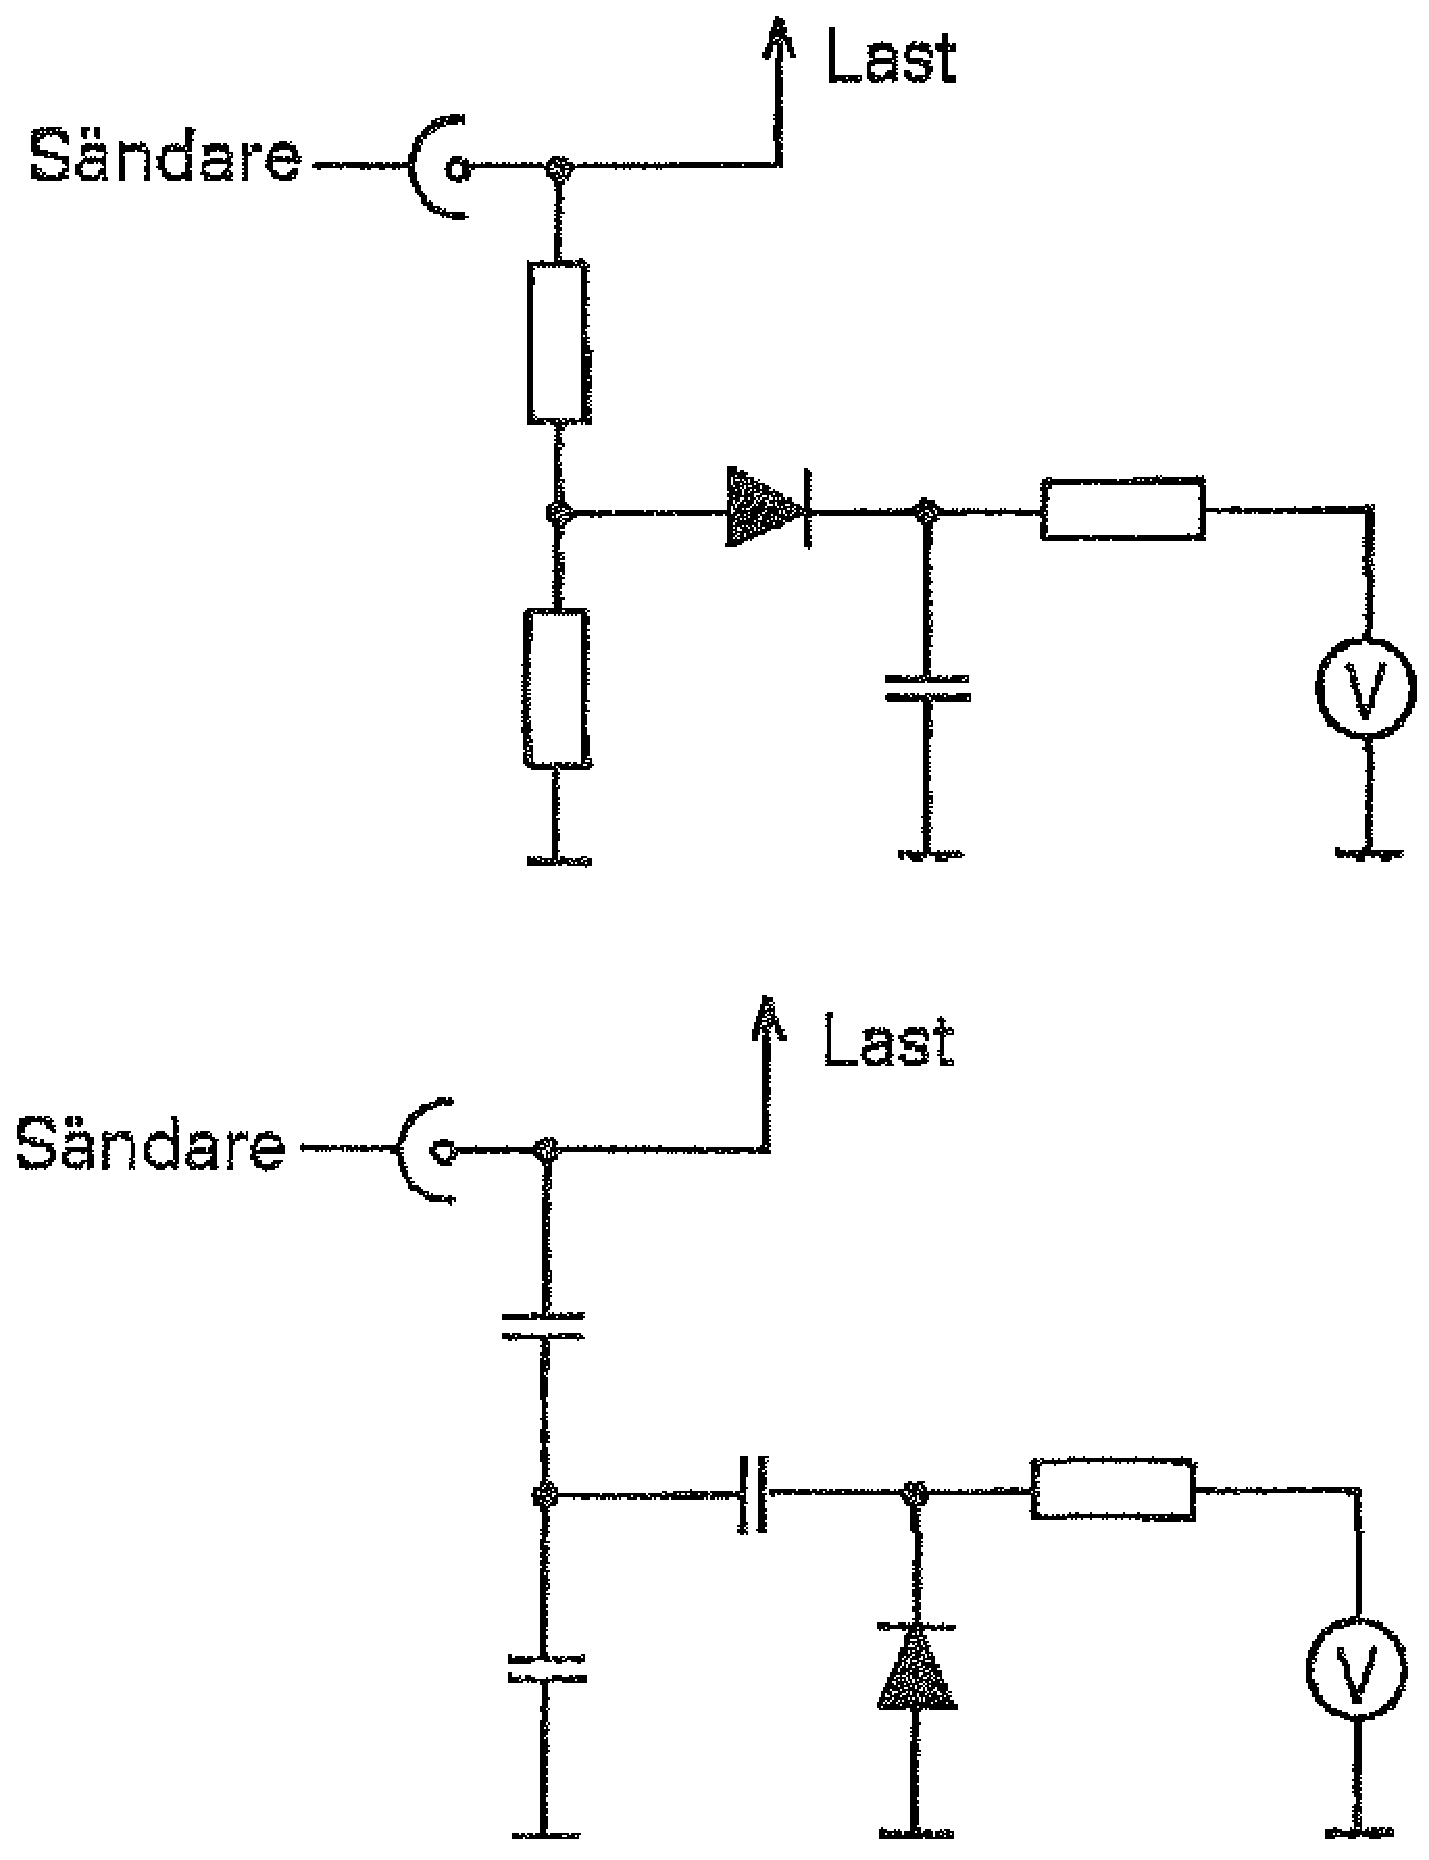
\includegraphics[width=0.5\textwidth]{images/cropped_pdfs/bild_2_8-01.pdf}
  \caption{Mätning av sändareffekt}
  \label{fig:bildII8-1}
\end{wrapfigure}

Bild \ref{fig:bildII8-1} visar en voltmeter med likriktare, som kopplats till
en sändare över spänningsdelare.
Två alternativa delare visas; den ena består av resistorer och den andra av
kondensatorer.

Den resistiva delaren är bättre i den meningen att den är frekvensoberoende och
inte belastar sändaren kapacitivt.
Dessutom dämpas övertoner som bildas vid likriktningen.
I den kapacitiva delaren kan övertoner passera lättare.

Denna mätmetod är noggrann bara när impedansen är lika i sändaren,
kabeln till lasten och själva lasten.
Lasten kan vara en konstlast, en antenn etc. och ska ha ett känt värde för att
effekten ska kunna beräknas.

Ett sätt att skaffa underlag för beräkning av PEP-effekten är att mäta
HF-strömmen med ett termokorsinstrument och spänningen med en
toppvärdesvisande voltmeter.
Utifrån dessa värden beräknar man effekten.
Denna metod är dock inte så vanlig.

\subsection{Direktvisande effektmetrar}
\textbf{
HAREC a.\ref{HAREC.a.8.2.1.2}\label{myHAREC.a.8.2.1.2}
}

Många föredrar direktvisande effektmätare.
En HF-voltmeter kan givetvis graderas för att visa effekt i stället för
spänning, men då med den viktiga förutsättningen att impedansen måste ha en
fastställt värde.

Om man avläser effekten genom en 75~\(\Omega\)-kabel på ett instrument för
50~\(\Omega\), så är det verkliga värdet ett annat än den avlästa.

De effektmetrar som förekommer i SVF-instrument är egentligen voltmetrar,
men med skalan graderad i effekt.

\subsection{Mäta ståendevågförhållande (SVF)}
\textbf{
HAREC a.\ref{HAREC.a.8.1.5}\label{myHAREC.a.8.1.5}
}
\label{mäta ståendevåg}
\label{ståendevågförhållande (SVF)}
\label{Standing Wave Ratio (SWR)}

När till exempel en antennledning ansluts till en antenn och deras impedanser
inte är lika, så kommer en del av inmatade effekten i ledningen att
reflekteras tillbaka från antennen.

Det uppstår då en stående våg i ledningen. Förhållandet mellan inmatad
och reflekterad effekt uttrycks som ett \emph{ståendevågförhållande (SVF)}
(eng. \emph{Standing Wave Ratio (SWR)}).

Med en SVF-meter som sätts in mellan effektkälla och ledning kan man
mäta hur stor effekt som matas in i ledningen och hur stor effekt som
vänder tillbaka från slutet av ledningen.

SVF-värdet kan bestämmas på något av följande sätt:
\begin{itemize}
\item Man mäter framåt- respektive bakåtgående effekt var för sig med
  en riktningskänslig effektmeter.
  Man beräknar därefter SVF eller tar fram det ur ett diagram.
\item Man använder ett instrument som beräknar eller visar SVF på något sätt.
\end{itemize}

\subsection{Studera vågformen}
\textbf{
HAREC a.\ref{HAREC.a.8.1.6}\label{myHAREC.a.8.1.6}
}

Vågformen för snabba växelströmsförlopp studeras bäst med oscilloskop.

\subsection{Mäta frekvens}
\textbf{
HAREC a.\ref{HAREC.a.8.1.7}\label{myHAREC.a.8.1.7}
}

Frekvensmätning gör man bäst med en s.k. frekvensräknare, som är ett
digitalt instrument.
Man kan också använda en s.k. absorbtionsvågmeter, som är mycket enkel och
inte alls lika exakt.
Vid frekvensmätning ansluter man instrumentet till mätobjektet med en
svag elektrisk eller magnetisk koppling.

\subsection{Mäta resonansfrekvens}
\textbf{
HAREC a.\ref{HAREC.a.8.1.8}\label{myHAREC.a.8.1.8}
}

Mäta resonansfrekvensen för en passiv svängningskrets gör man klassiskt
med en så kallad dip-meter.
Idag använder man antingen en spektrum-analysator med tracking-generator,
dvs. en SNA, eller en nätverksanalysator för att med bättre precision mäta
resonansfrekvenser.

\subsection{Mätfel}

Mätinstrument indelas i noggrannhetsklasser efter största tillåtna felvisning.
Klasserna är 0.1, 0.2, 0.5, 1.0, 1.5, 2.5 och 5.0 varvid klassen anges på
instrumentet.
Som exempel får ett instrument i klass 2.5 ha ett tillåtet mätfel av
\(\pm\)2,5~\% av fullt utslag.

Mätresultatet bestäms av flera faktorer; dels av instrumentets
s.k. mätonoggrannhet, dels av hur mätvärdet presenteras och slutligen
av hur noga användaren läser av.

Vid \emph{analog} visning presenteras mätvärdet med en visare mot en
graderad skala med en viss upplösning.
Visaren kan vara mekanisk eller optisk (ljusspalt).
Vid snabba mätvärdesändringar är instrumentets mekaniska tröghet en faktor
att ta hänsyn till.

Vid \emph{digital} visning presenteras mätvärdet med siffror eller som
längden på en pelare.
Det är förledande att se digital visning med siffror som mer exakt än analog,
men det är inte alls säkert.
Utöver instrumentets mätonoggrannhet, bestäms nämligen noggrannheten av hur
många siffror som mätresultatet presenteras i.

En oberäknelig källa till mätfel är elektromagnetiska fält från
apparater i närheten.

En ofta förbisedd felkälla är temperaturen i mätobjektet och/eller i
instrumentet, det kan vara av inkopplingstiden med mera.

\emph{Visningströgheten} är inget mätfel i sig men kan till nackdel
vid snabba förlopp.
Trögheten förekommer såväl vid analog som digital visning.
I det förra fallet är masströghet i instrumentets rörliga delar orsaken och i
det andra fallet är orsaken klockfrekvensen för instrumentets mikroprocessor.
